\documentclass[aps,pra,11pt,onecolumn,nofootinbib,tightenlines]{revtex4-2}

\usepackage{mathrsfs}
\usepackage{amsmath}
\usepackage{amsfonts}
\usepackage{amssymb}
\usepackage{amsthm}
\usepackage{tikz}
\usetikzlibrary{arrows.meta,positioning}
\usepackage{booktabs}
\usepackage{array}
\usepackage[colorlinks=true,urlcolor=blue,citecolor=blue,linkcolor=blue]{hyperref}
\usepackage{xurl}
\usepackage{natbib}

\newcommand{\LeanDecl}[1]{\path{#1}}
\newcommand{\Formalized}{\textup{Formalized}}
\newcolumntype{L}[1]{>{\raggedright\arraybackslash}p{#1}}
\newcommand{\StatementCell}[1]{\begin{minipage}[t]{0.25\textwidth}\vspace{0pt}\raggedright #1\end{minipage}}
\newcommand{\LeanCell}[1]{\begin{minipage}[t]{0.49\textwidth}\vspace{0pt}\raggedright #1\end{minipage}}
\newcommand{\StatusCell}[1]{\begin{minipage}[t]{0.18\textwidth}\vspace{0pt}\raggedright #1\end{minipage}}
\renewcommand{\thesection}{\arabic{section}}

\begin{document}

\title{Lean Formalization of the Parameter Classification for Conditional Entropies}

\begin{abstract}
This note explains how Lean~4 verifies the necessary and sufficient parameter
conditions for the concrete conditional-entropy candidates studied in the
complete-proof paper, Ref.~\cite{rubboli2026parametersFull}. The formalization
covers all thirty-one numbered results: sixteen results in Sections~4 and~5 and
fifteen technical results in Appendix~A. For each result, the note identifies
one distinct Lean theorem with the same mathematical content, allowing the
reader to move directly from a statement in the paper to its formal proof. A
dependency diagram also shows how the main classification is built from the
underlying calculus, measure-theoretic, localization, and semiring/channel
results. Every supporting result is proved using Lean and Mathlib: the
development contains no unfinished proofs, project-defined axioms, or
additional unproved assumptions. No previous knowledge of Lean is needed to
understand the organization of the formalization described here.
\end{abstract}

\author{Roberto Rubboli}
\noaffiliation
\author{Erkka Haapasalo}
\noaffiliation
\author{Marco Tomamichel}
\noaffiliation

\maketitle

\section{Lean correspondence}
\label{sec:lean-correspondence}

The formal development follows the complete analytic proofs in
Ref.~\cite{rubboli2026parametersFull}. It covers the endpoint-aware R\'enyi parameter,
real-power and entropy differentiation, signed integration, common
discretization, the two-block, three-block, and Shannon localizers, exact
tropical stationarity, all sufficiency and necessity branches, and the
original finite semiring and conditionally mixing channel lift. The source is
available at
\url{https://github.com/robertorubboli/A-complete-characterization-of-conditional-entropies}
on the repository's main branch.

Throughout this note, every numbered lemma, proposition, or remark uses the
number in the complete-proof paper,
Ref.~\cite{rubboli2026parametersFull}. That paper alone determines the
organization, numbering, and conventions of the Lean correspondence.

There are two terminal conclusions. The declaration
\LeanDecl{mainClassification} says that, for every probability measure on the
compactified R\'enyi parameter space, monotonicity of each concrete candidate
is equivalent to its exact admissibility condition. Its only explicit argument
is the measure being classified; it has no auxiliary hypothesis. The closed
declaration \LeanDecl{allConditionalEntropyAxioms} proves nonnegativity,
zero-embedding invariance, tensor additivity, fair-bit normalization, and
embedded channel monotonicity for every admissible candidate. Neither theorem
assumes a project-specific axiom. In the complete-proof paper and in Lean,
$\log$ is the natural logarithm and an independent fair bit has value $\log 2$.

The repository contains two complementary dependency diagrams at different
levels of detail. Figure~\ref{fig:lean-dependencies} is the \emph{theorem-facing proof
map}: it connects public conclusions to numbered complete-proof results and
reusable proof ingredients. It is not a module-import graph. The standalone
files \path{paper/dependency-graph.dot}, \path{paper/dependency-graph.svg}, and
\path{paper/dependency-graph.png} are three formats of one detailed
\emph{Lean implementation dependency graph}; their arrows run from prerequisite
to dependent.

In Figure~\ref{fig:lean-dependencies}, arrows deliberately point in the reverse
direction, from a conclusion to ingredients used in its proof. Pale green boxes
are the two public conclusions, white boxes are paper-facing intermediate
results, and pale blue boxes are reusable infrastructure that is itself proved
in Lean.

\begin{figure}[htbp]
\centering
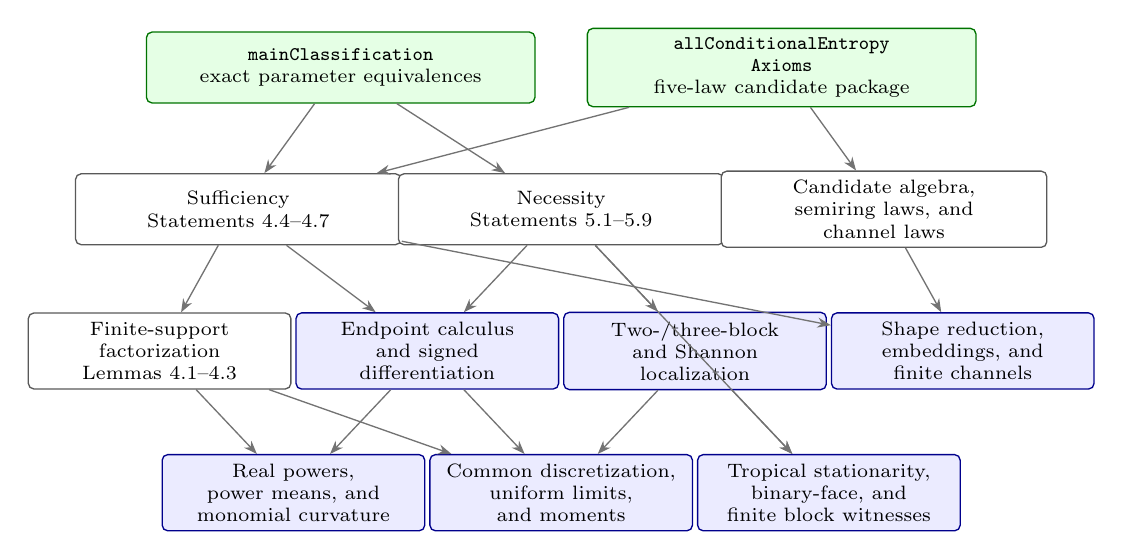
\begin{tikzpicture}[
  >=Stealth,
  every path/.style={draw=black!55,line width=.48pt,-{Stealth[length=1.7mm]}},
  final/.style={draw=green!45!black,fill=green!10,rounded corners=2pt,
    align=center,font=\scriptsize,text width=47mm,minimum height=9mm},
  paper/.style={draw=black!65,fill=white,rounded corners=2pt,
    align=center,font=\scriptsize,text width=39mm,minimum height=9mm},
  infra/.style={draw=blue!55!black,fill=blue!8,rounded corners=2pt,
    align=center,font=\scriptsize,text width=31mm,minimum height=9mm},
  papercompact/.style={draw=black!65,fill=white,rounded corners=2pt,
    align=center,font=\scriptsize,text width=31mm,minimum height=9mm}]

\node[final] (classification) at (-2.8,0)
  {\texttt{mainClassification}\\exact parameter equivalences};
\node[final] (laws) at (2.8,0)
  {\texttt{allConditionalEntropy}\\\texttt{Axioms}\\five-law candidate package};

\node[paper] (suff) at (-4.1,-1.8)
  {Sufficiency\\Statements~4.4--4.7};
\node[paper] (necess) at (0,-1.8)
  {Necessity\\Statements~5.1--5.9};
\node[paper] (candidate) at (4.1,-1.8)
  {Candidate algebra,\\semiring laws, and\\channel laws};

\node[papercompact] (finite) at (-5.1,-3.6)
  {Finite-support\\factorization\\Lemmas~4.1--4.3};
\node[infra] (endpoint) at (-1.7,-3.6)
  {Endpoint calculus\\and signed\\differentiation};
\node[infra] (local) at (1.7,-3.6)
  {Two-/three-block\\and Shannon\\localization};
\node[infra] (channel) at (5.1,-3.6)
  {Shape reduction,\\embeddings, and\\finite channels};

\node[infra] (powers) at (-3.4,-5.4)
  {Real powers,\\power means, and\\monomial curvature};
\node[infra] (disc) at (0,-5.4)
  {Common discretization,\\uniform limits,\\and moments};
\node[infra] (stationary) at (3.4,-5.4)
  {Tropical stationarity,\\binary-face, and\\finite block witnesses};

\draw (classification) -- (suff);
\draw (classification) -- (necess);
\draw (laws) -- (suff);
\draw (laws) -- (candidate);
\draw (suff) -- (finite);
\draw (suff) -- (endpoint);
\draw (suff) -- (channel);
\draw (necess) -- (endpoint);
\draw (necess) -- (local);
\draw (necess) -- (stationary);
\draw (candidate) -- (channel);
\draw (finite) -- (powers);
\draw (finite) -- (disc);
\draw (endpoint) -- (powers);
\draw (endpoint) -- (disc);
\draw (local) -- (disc);
\draw (local) -- (stationary);
\end{tikzpicture}
\caption{Theorem-facing proof map for the parameter classification. Every
displayed statement number is from the complete-proof paper,
Ref.~\cite{rubboli2026parametersFull}. Arrows point from a result to ingredients used in its proof, the
reverse of the prerequisite-to-dependent convention in the detailed Lean
implementation dependency graph. Color
records proof role, not confidence: green means public conclusion, blue means
internally proved infrastructure, and white means a paper-facing result.}
\label{fig:lean-dependencies}
\end{figure}

Table~\ref{tab:lean-correspondence} follows the numbering of the complete-proof
paper, Ref.~\cite{rubboli2026parametersFull}.  It is a one-to-one index at the
paper-facing interface: each of the sixteen numbered environments in the
main text, including Remarks~5.4--5.5, has exactly one distinct canonical Lean
declaration, and no declaration in the table represents two manuscript
environments.  All names are in the namespace
\LeanDecl{ConditionalEntropy} and are defined in
\path{ConditionalEntropy/FullDetailsStatements.lean}.  A canonical declaration
may use several smaller lemmas internally.  Those implementation dependencies
are not additional entries in the correspondence and are recorded separately
in the source and dependency graph.

This interface-level bijection says exactly which Lean theorem a reader should
inspect for each manuscript result; it does not claim that the internal proof
graph is one-to-one.

\renewcommand{\arraystretch}{1.12}
\begin{table}[htbp]
\centering
\small
\caption{Statement-by-statement correspondence. All numbers are from the
complete-proof paper, Ref.~\cite{rubboli2026parametersFull}.}
\label{tab:lean-correspondence}
\begin{tabular}{@{}lll@{}}
\toprule
\StatementCell{\textbf{Manuscript statement}} &
\LeanCell{\textbf{Lean declaration}} & \StatusCell{\textbf{Status}}\\
\midrule
\StatementCell{Lemma~4.1: Power-mean curvature} &
\LeanCell{\LeanDecl{fullDetailsLemma4_1}} &
\StatusCell{Exact}\\
\addlinespace
\StatementCell{Lemma~4.2: Monomial curvature} &
\LeanCell{\LeanDecl{fullDetailsLemma4_2}} &
\StatusCell{Exact}\\
\addlinespace
\StatementCell{Lemma~4.3: Finite-support sufficiency} &
\LeanCell{\LeanDecl{fullDetailsLemma4_3}} &
\StatusCell{Exact}\\
\addlinespace
\StatementCell{Proposition~4.4: General temperate sufficiency} &
\LeanCell{\LeanDecl{fullDetailsProposition4_4}} &
\StatusCell{Exact}\\
\addlinespace
\StatementCell{Proposition~4.5: Negative-tropical sufficiency} &
\LeanCell{\LeanDecl{fullDetailsProposition4_5}} &
\StatusCell{Exact}\\
\addlinespace
\StatementCell{Proposition~4.6: Positive-tropical sufficiency} &
\LeanCell{\LeanDecl{fullDetailsProposition4_6}} &
\StatusCell{Exact}\\
\bottomrule
\end{tabular}
\end{table}

\begin{table}[htbp]
\centering
\small
\textbf{Table~\ref{tab:lean-correspondence} (continued; complete-proof numbering).}\par\smallskip
\begin{tabular}{@{}lll@{}}
\toprule
\StatementCell{\textbf{Manuscript statement}} &
\LeanCell{\textbf{Lean declaration}} & \StatusCell{\textbf{Status}}\\
\midrule
\StatementCell{Proposition~4.7: Derivation sufficiency} &
\LeanCell{\LeanDecl{fullDetailsProposition4_7}} &
\StatusCell{Exact}\\
\addlinespace
\StatementCell{Proposition~5.1: Positive necessity} &
\LeanCell{\LeanDecl{fullDetailsProposition5_1}} &
\StatusCell{Exact}\\
\addlinespace
\StatementCell{Proposition~5.2: Negative Shannon atom excludes upper support} &
\LeanCell{\LeanDecl{fullDetailsProposition5_2}} &
\StatusCell{Exact}\\
\addlinespace
\StatementCell{Proposition~5.3: Truncated exceptional-moment bound} &
\LeanCell{\LeanDecl{fullDetailsProposition5_3}} &
\StatusCell{Exact}\\
\bottomrule
\end{tabular}
\end{table}

\begin{table}[htbp]
\centering
\small
\textbf{Table~\ref{tab:lean-correspondence} (continued; complete-proof numbering).}\par\smallskip
\begin{tabular}{@{}lll@{}}
\toprule
\StatementCell{\textbf{Manuscript statement}} &
\LeanCell{\textbf{Lean declaration}} & \StatusCell{\textbf{Status}}\\
\midrule
\StatementCell{Remark~5.4: Unnormalised cone witnesses and homogeneity} &
\LeanCell{\LeanDecl{fullDetailsRemark5_4}} &
\StatusCell{Exact}\\
\addlinespace
\StatementCell{Remark~5.5: Compensated two-column witness} &
\LeanCell{\LeanDecl{fullDetailsRemark5_5}} &
\StatusCell{Exact}\\
\addlinespace
\StatementCell{Proposition~5.6: Exceptional negative branch: unique upper
point, finite one-sided moments, and moment bound} &
\LeanCell{\LeanDecl{fullDetailsProposition5_6}} &
\StatusCell{Exact}\\
\bottomrule
\end{tabular}
\end{table}

\begin{table}[htbp]
\centering
\small
\textbf{Table~\ref{tab:lean-correspondence} (continued; complete-proof numbering).}\par\smallskip
\begin{tabular}{@{}lll@{}}
\toprule
\StatementCell{\textbf{Manuscript statement}} &
\LeanCell{\textbf{Lean declaration}} & \StatusCell{\textbf{Status}}\\
\midrule
\StatementCell{Proposition~5.7: Negative-tropical necessity} &
\LeanCell{\LeanDecl{fullDetailsProposition5_7}} &
\StatusCell{Exact}\\
\addlinespace
\StatementCell{Proposition~5.8: Positive-tropical necessity} &
\LeanCell{\LeanDecl{fullDetailsProposition5_8}} &
\StatusCell{Exact}\\
\addlinespace
\StatementCell{Proposition~5.9: Derivation necessity} &
\LeanCell{\LeanDecl{fullDetailsProposition5_9}} &
\StatusCell{Exact}\\
\bottomrule
\end{tabular}
\end{table}

\clearpage

Table~\ref{tab:lean-correspondence} is the stable reader-facing interface.
Each facade may call several lower-level lemmas, but those implementation
dependencies do not create additional manuscript correspondences.

The repository also keeps a machine-readable 31-row audit of every numbered
environment in the complete-proof document, including Appendix~A, in
\path{paper/full-details-correspondence.json}.  Appendix statements are
listed separately below because they provide technical ingredients rather
than the main Section~4--5 conclusions.  The much larger 152-row internal
formalization-blueprint ledger and the editable Lean implementation dependency
graph serve still different purposes and are not part of this bijection.

Table~\ref{tab:lean-appendix-correspondence} completes the index for the
fifteen numbered Appendix statements, all of which have exact facades.
Row~A.9 bundles joint entropy-line continuity with the exact cancellation
integral for orders zero, one, and two. Thus every row in the two tables is
exact.

\begin{table}[htbp]
\centering
\small
\caption{Appendix statement correspondence.  All numbers are from Appendix~A
of the complete-proof paper, Ref.~\cite{rubboli2026parametersFull}.}
\label{tab:lean-appendix-correspondence}
\begin{tabular}{@{}lll@{}}
\toprule
\StatementCell{\textbf{Manuscript statement}} &
\LeanCell{\textbf{Lean declaration}} & \StatusCell{\textbf{Status}}\\
\midrule
\StatementCell{Lemma~A.1: Hessian of the power mean} &
\LeanCell{\LeanDecl{fullDetailsAppendixA_1}} &
\StatusCell{Exact}\\
\addlinespace
\StatementCell{Lemma~A.2: Hessian and sign classification of a monomial} &
\LeanCell{\LeanDecl{fullDetailsAppendixA_2}} &
\StatusCell{Exact}\\
\addlinespace
\StatementCell{Lemma~A.3: Continuity and uniform bound for finite-dimensional R\'enyi entropy} &
\LeanCell{\LeanDecl{fullDetailsAppendixA_3}} &
\StatusCell{Exact}\\
\addlinespace
\StatementCell{Lemma~A.4: Concavity and Schur concavity in the sufficient-condition ranges} &
\LeanCell{\LeanDecl{fullDetailsAppendixA_4}} &
\StatusCell{Exact}\\
\bottomrule
\end{tabular}
\end{table}

\begin{table}[htbp]
\centering
\small
\textbf{Table~\ref{tab:lean-appendix-correspondence} (continued).}\par\smallskip
\begin{tabular}{@{}lll@{}}
\toprule
\StatementCell{\textbf{Manuscript statement}} &
\LeanCell{\textbf{Lean declaration}} & \StatusCell{\textbf{Status}}\\
\midrule
\StatementCell{Lemma~A.5: Measure-theoretic tools} &
\LeanCell{\LeanDecl{fullDetailsAppendixA_5}} &
\StatusCell{Exact}\\
\addlinespace
\StatementCell{Lemma~A.6: Common discrete approximation of the R\'enyi parameter} &
\LeanCell{\LeanDecl{fullDetailsAppendixA_6}} &
\StatusCell{Exact}\\
\addlinespace
\StatementCell{Lemma~A.7: Pointwise limits preserve the shape inequalities} &
\LeanCell{\LeanDecl{fullDetailsAppendixA_7}} &
\StatusCell{Exact}\\
\addlinespace
\StatementCell{Lemma~A.8: First and second derivatives of the logarithmic power mean} &
\LeanCell{\LeanDecl{fullDetailsAppendixA_8}} &
\StatusCell{Exact}\\
\bottomrule
\end{tabular}
\end{table}

\begin{table}[htbp]
\centering
\small
\textbf{Table~\ref{tab:lean-appendix-correspondence} (continued).}\par\smallskip
\begin{tabular}{@{}lll@{}}
\toprule
\StatementCell{\textbf{Manuscript statement}} &
\LeanCell{\textbf{Lean declaration}} & \StatusCell{\textbf{Status}}\\
\midrule
\StatementCell{Lemma~A.9: Cancellation and continuity through the Shannon point} &
\LeanCell{\LeanDecl{fullDetailsAppendixA_9}} &
\StatusCell{Exact}\\
\addlinespace
\StatementCell{Lemma~A.10: Continuity of the differentiated entropy at the parameter endpoints} &
\LeanCell{\LeanDecl{fullDetailsAppendixA_10}} &
\StatusCell{Exact}\\
\addlinespace
\StatementCell{Proposition~A.11: Differentiation under the R\'enyi-parameter integral at fixed dimension} &
\LeanCell{\LeanDecl{fullDetailsAppendixA_11}} &
\StatusCell{Exact}\\
\addlinespace
\StatementCell{Lemma~A.12: Dominant-block remainder} &
\LeanCell{\LeanDecl{fullDetailsAppendixA_12}} &
\StatusCell{Exact}\\
\bottomrule
\end{tabular}
\end{table}

\begin{table}[htbp]
\centering
\small
\textbf{Table~\ref{tab:lean-appendix-correspondence} (continued).}\par\smallskip
\begin{tabular}{@{}lll@{}}
\toprule
\StatementCell{\textbf{Manuscript statement}} &
\LeanCell{\textbf{Lean declaration}} & \StatusCell{\textbf{Status}}\\
\midrule
\StatementCell{Lemma~A.13: First two derivatives of Shannon entropy along an affine path} &
\LeanCell{\LeanDecl{fullDetailsAppendixA_13}} &
\StatusCell{Exact}\\
\addlinespace
\StatementCell{Lemma~A.14: Second-order condition for a one-dimensional quasi-convex function} &
\LeanCell{\LeanDecl{fullDetailsAppendixA_14}} &
\StatusCell{Exact}\\
\addlinespace
\StatementCell{Lemma~A.15: Exact finite-dimensional stationarity correction} &
\LeanCell{\LeanDecl{fullDetailsAppendixA_15}} &
\StatusCell{Exact}\\
\bottomrule
\end{tabular}
\end{table}

\clearpage
\subsection{Trust boundary and reproducibility}

The project is pinned to Lean~4.32.2 and Mathlib~4.32.2. The release source
contains no \texttt{sorry}, \texttt{admit}, project-defined \texttt{axiom}, or
project-defined \texttt{opaque} declaration. The final declarations contain no
unproved project hypothesis. Lean's standard logical foundations, including
classical choice, propositional extensionality, and quotient soundness, remain
part of the ordinary trusted base.

The single command
\begin{verbatim}
powershell -File scripts/check.ps1
\end{verbatim}
runs the forbidden-token scan, a warning-as-error build of the integrated
\LeanDecl{CompleteCharacterization} target, the axiom audit, and a structural
audit of the internal 152-row blueprint ledger.  It also runs the independent
full-details audit, which reconstructs all thirty-one numbers and labels from
the LaTeX source, checks that canonical names are unique and in the recorded
order, and asks Lean to elaborate every exact declaration.  The
formalization proves the classification and law package for the four concrete
candidate families in the complete-proof paper's natural-log convention.

\bibliographystyle{ultimate}
\renewcommand{\bibfont}{\footnotesize}
\bibliography{bibliography}

\end{document}
